\documentclass{article}
\usepackage[T1]{fontenc}

\usepackage{graphicx}
\usepackage{etoolbox}
\newcommand{\icon}[1]{\includegraphics[height=17pt]{#1}}
\robustify{\icon}

\usepackage{bm}
\usepackage{lmodern}
\usepackage{float} 
\usepackage{setspace}
\usepackage[svgnames]{xcolor} % Required for colour specification
\usepackage{enumitem}
\usepackage{listings}
\usepackage{color,colortbl}
\definecolor{scnumber}{RGB}{166,34,158}

\usepackage{varioref}
\usepackage[square]{natbib}

\usepackage{hyperref}
\hypersetup{colorlinks=true,linkcolor={black},citecolor={black}}

\newcommand{\myuline}[1]{%
  \uline{\phantom{#1}}%
  \llap{\contour{white}{#1}}%
}

\usepackage{lettrine}
\usepackage{ragged2e}
\usepackage{textcomp}
\usepackage{sclang}

\newcommand\digitstyle{\color{scnumber}}
\makeatletter
\newcommand{\ProcessDigit}[1]
{%
  \ifnum\lst@mode=\lst@Pmode\relax%
   {\digitstyle #1}%
  \else
    #1%
  \fi
}
\makeatother
\lstset{literate=
   % {'} {\textquotesingle}1
    {0}{{{\ProcessDigit{0}}}}1
    {1}{{{\ProcessDigit{1}}}}1
    {2}{{{\ProcessDigit{2}}}}1
    {3}{{{\ProcessDigit{3}}}}1
    {4}{{{\ProcessDigit{4}}}}1
    {5}{{{\ProcessDigit{5}}}}1
    {6}{{{\ProcessDigit{6}}}}1
    {7}{{{\ProcessDigit{7}}}}1
    {8}{{{\ProcessDigit{8}}}}1
    {9}{{{\ProcessDigit{9}}}}1,
    %{<=}{{\(\leq\)}}1	
   % {~} {$\sim$}1,
%    morestring=[b]",
%    morestring=[b]',
%    morecomment=[l]//,
%    stringstyle=\color{scstring},
%    commentstyle=\color{sccomment},
%    morekeywords=[2]{thisProcess},
%    keywordstyle=[2]\color{scspecial},
%    morekeywords=[4]{vOst, xt},
%    keywordstyle=[4]\color{scvar},
%    morekeywords=[3]{NetAddr, OSCdef},
%    keywordstyle=[3]\color{scclass},
%    morekeywords=[5]{ostinato, recvPort, netaddr},
%    keywordstyle=[5]\color{scsymbol},
%    moredelim=[s][\color{scvar}]{\ ~}{\ },
%    moredelim=[s][\color{scvar}]{\ ~}{e},
%    basicstyle=\ttfamily\footnotesize,
%    showstringspaces=false,	
}

\lstdefinelanguage{inscore}{
    language=Bash,
    literate=%
    {'} {\textquotesingle}1
    {0}{{{\color{black}0}}}1
    {1}{{{\color{black}1}}}1
    {2}{{{\color{black}2}}}1
    {3}{{{\color{black}3}}}1
    {4}{{{\color{black}4}}}1
    {5}{{{\color{black}5}}}1
    {6}{{{\color{black}6}}}1
    {7}{{{\color{black}7}}}1
    {8}{{{\color{black}8}}}1
    {9}{{{\color{black}9}}}1,
    stringstyle=\color{black},
    commentstyle=\color{gray},
    numberstyle=\color{black},
    showstringspaces=false,
    basicstyle=\ttfamily\scriptsize,
    }
    
\usepackage{enumitem}
\definecolor{sccomment}{RGB}{113, 113, 113}
\definecolor{scclass}{RGB}{38, 97, 177}
\definecolor{sclink}{RGB}{46, 21, 193}

\usepackage{subcaption}
\usepackage{moresize}

\begin{document}

\begin{center}
\section*{\huge\sffamily INScore ... in action}
\vspace{-0.3cm}
\textsl{An environment for the design of interactive,}

\textsl{augmented, dynamic musical scores.}

\href{https://inscore.grame.fr}{\texttt{\small https://inscore.grame.fr}}

\vspace{0.3cm} 

%\icon{sc}
\begin{figure}[htbp]
\begin{center}

\includegraphics[width=1.5cm]{sc}
\end{center}
\end{figure}
\texttt{October 21, 2024}
%\subsubsection*{Yann Ics\\Conceptual Composer\\\texttt{\small by.cmsc@gmail.com}}

\href{https://scsynth.org/u/Yann\_Ics}{\texttt{\small https://scsynth.org/u/Yann\_Ics}}

\end{center}
\vspace{0.2cm}


\begin{center}
\texttt{\footnotesize INScore version 1.31}
 
 \vspace{-0.1cm}
\texttt{\footnotesize SuperCollider version 3.13.0}
\end{center}

\vspace{0.7cm}

%\section*{Preamble}
%In the SuperCollider context, writing a score can be very challenging because of the tricky syntax (Lilypond versus MusicXML) versus the user's required rendering and preferences. SC (SuperCollider) is then intended to generate a score either to show what it is played (more or less in real-time mode) or what it is going to be played (by a performer for instance) once the score is available. The latter cannot be well formatted because we face too many parameters and possible collusions to output a perfect partition in one shot. We have to be conscious of that and manage with that. Each user has to find by him/herself some adjustments, even to manage case by case each issue `by hand'. Maybe the outcome of this observation is a compromise like ... INScore and its related Guido engine notation, which proposes a reliable and efficient way for writing and displaying scores even in real-time mode.

%\smallskip

%\noindent \rule{\linewidth}{.5pt}

\bfseries
\lettrine[lhang=.03]{T}{his} short article aims to illustrate one way to use the open-source software INScore, like a tutorial introduction within the SuperCollider context. Furthermore, this could be the first step toward developing an interface as an extension of SuperCollider.

 \mdseries
 \smallskip
%\section*{Resources}
%
%$\rightarrow$ \href{https://inscore.grame.fr}{\texttt{\small https://inscore.grame.fr}}

%\vspace{0.7cm}
\begin{center}
  $\ast$~$\ast$~$\ast$
\end{center}

%\section*{Localhost}
\subsection*{Here is the context}
I am studying on a musical project named \textit{Untitled} \texttt{\#2} developed in SuperCollider as an algorithmic and synthesis composition. In short,
a third-party application generates a melody based on the dynamic Markov chain and an \textit{ostinato} as an emergent phenomenon due to the structure of a resulting network. This said application is about an AI developed in Common Lisp called \textsl{Neuromuse3} based on a connectionism network and trained with the encoded voices of the first book of J. S. Bach’s \textit{Das Wohltemperirte Klavier} (BWV 846 – 869). All these data are sent via the OSC protocol. Then SuperCollider interprets them musically via different syntheses. A GUI mixer allows one to formalize the work in a real-time performance. 

From this point, I imagined that one musician performer could interact by improvising according to some guidelines displayed through the INScore viewer.% via OSC communication.
 What should shown is the harmonic context (\textit{in-time} with a before and an after to anticipate the oncoming) as note names plus optional transitional notes, and the rhythm related to this event. So, there is no direct interaction with INScore, only indications to serve the musician playing. 

\begin{center}
  $\ast$~$\ast$~$\ast$
\end{center}

\subsection*{The coding part}
 

Beforehand, to initialize the INScore display, some preliminary setup needs to be written on a file to be loaded remotely. These setups mainly consist of positioning each object related to each other. Although this can be done dynamically from a third-party application via OSC messages.

\begin{lstlisting}[language=inscore]
# clear the scene
/ITL/scene/* del;
/ITL/scene width 1;
# ---
/ITL/scene/timing set txt "The upper numeral of the time signature gives you
 the timing in second."; 
/ITL/scene/timing y -0.6;
/ITL/scene/timing scale 0.8;
/ITL/scene/tempo set txt "Tempo libre"; 
/ITL/scene/tempo y -0.53;
# harmony
# --- previous
/ITL/scene/a1 set txt "";
/ITL/scene/a1 scale 3;
/ITL/scene/a1 color 'orange';
/ITL/scene/a1 y -0.15;
/ITL/scene/a1 x -0.55;
# --- transitional previous
/ITL/scene/a2 set txt "";
/ITL/scene/a2 scale 2;
/ITL/scene/a2 color 'red';
/ITL/scene/a2 y -0.05;
/ITL/scene/a2 x -0.3;
# --- current
/ITL/scene/a3 set txt "";
/ITL/scene/a3 scale 3;
/ITL/scene/a3 y -0.15;
/ITL/scene/a3 x 0;
# --- transitional next
/ITL/scene/a4 set txt "";
/ITL/scene/a4 scale 2;
/ITL/scene/a4 color 'red';
/ITL/scene/a4 y -0.05;
/ITL/scene/a4 x 0.3;
# --- next
/ITL/scene/a5 set txt "";
/ITL/scene/a5 scale 3;
/ITL/scene/a5 color 'orange';
/ITL/scene/a5 y -0.15;
/ITL/scene/a5 x 0.55;
# rhythm (pause)
/ITL/scene/rtm set gmn '[ \meter<"">  \staffFormat<style="1-line"> 
 \clef<"perc"> \fermata<"long">(_/1) | empty*1/32 \staffOff ]';
/ITL/scene/rtm y 0.4;
/ITL/scene/rtm scale 0.8;
# set scene font
/ITL/scene/* fontFamily Courier;
\end{lstlisting}

\noindent  Each line is defined by the discriminant or tag \texttt{/ITL/}, the name of the scene, i.e. the window viewer, plus an identifier, followed by a keyword and its parameter(s) if required, which are well documented with examples in the INScore application folder as PDF and INScore files. Here, only the lines concerning the text of harmony and the score \texttt{gmn} (acronym of guido musical notation) will be dynamically set according to the context. The code is saved (in a file named \texttt{ics.inscore} currently) and must be loaded in a remote server (from the INScore API) in order to be accessible from any device.

\bigskip

\noindent %Data conditions the score display to be played inside a given duration shown in the first line. 
The score consists of displaying in the INScore viewer the previous harmony, the current harmony, and the next harmony plus the passing notes as a set of note names, and the rhythm partition.

 
%\begin{figure}[htbp]
%\begin{center}
%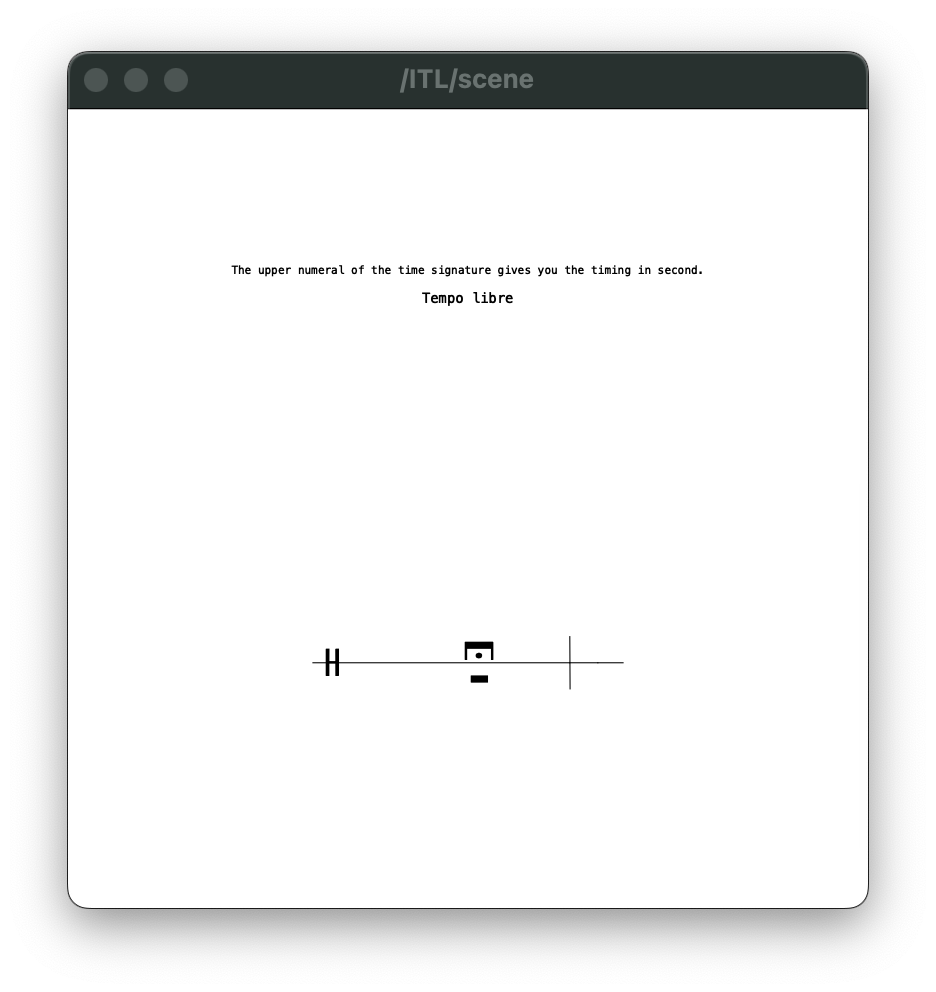
\includegraphics[width=5cm]{init.png}
%\caption{...}
%\end{center}
%\end{figure}


\begin{figure}[h]

\begin{subfigure}{0.5\textwidth}
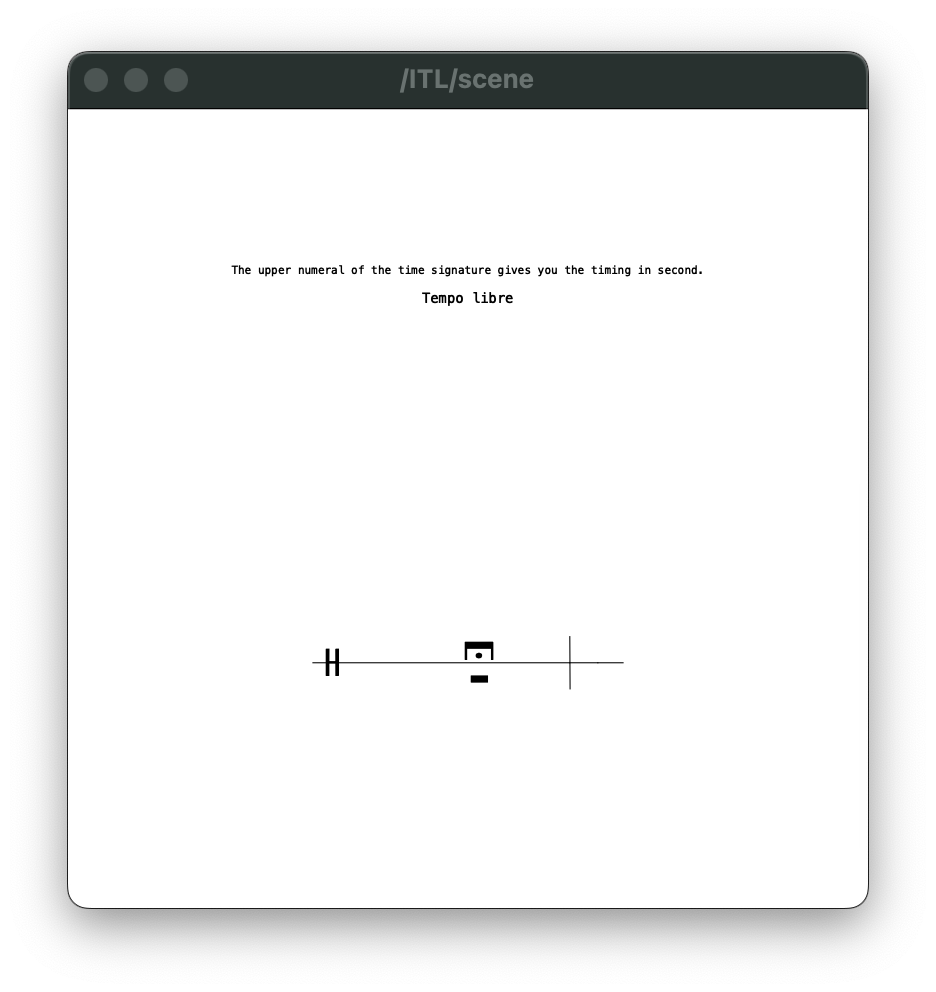
\includegraphics[width=0.9\linewidth, height=6cm]{init} 
\caption{initialization and waiting state ...}
\label{fig:init}
\end{subfigure}
\begin{subfigure}{0.5\textwidth}
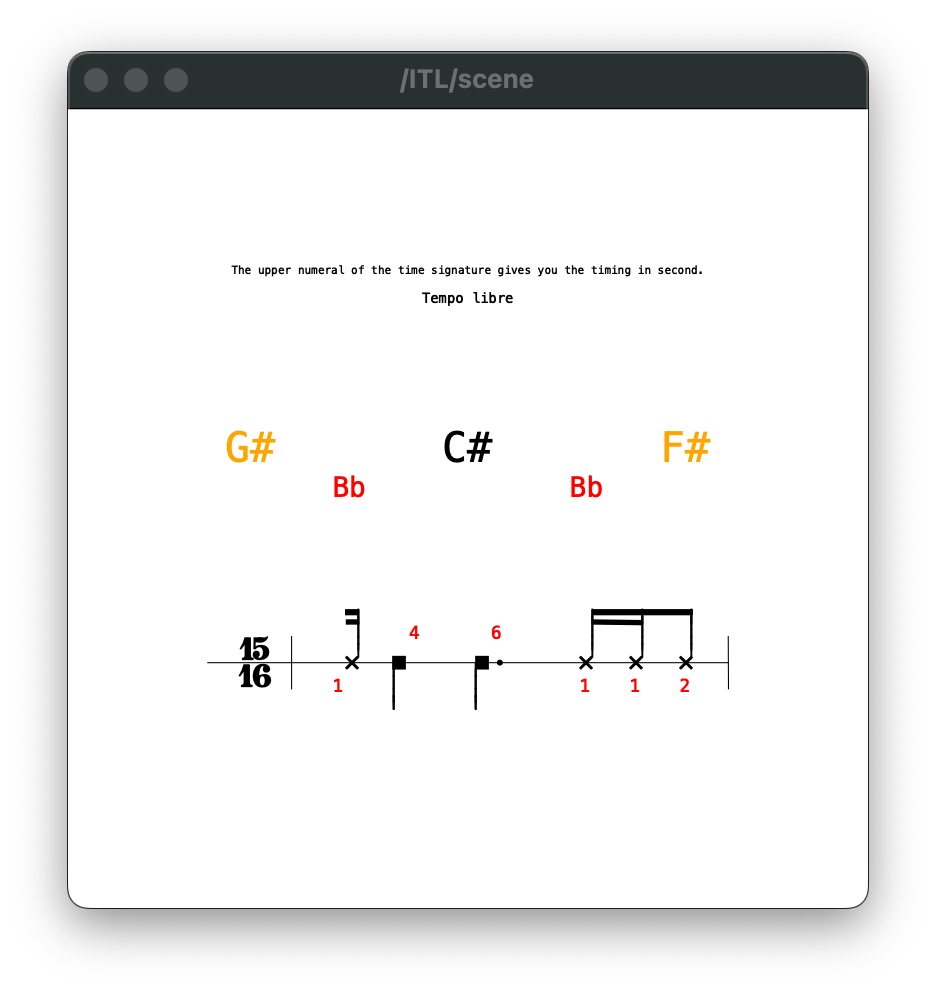
\includegraphics[width=0.9\linewidth, height=6cm]{ins1}
\caption{... in action ...}
\label{fig:ins1}
\end{subfigure}

\caption{This is what should be displayed on the musician's device.}
\label{fig:insviewer}
\end{figure}

\noindent On the SuperCollider side, I receive data from a third-party application -- namely \textsl{Neuromuse3}. 
\begin{lstlisting}[style=SuperCollider-IDE]
// opening incoming port
thisProcess.openUDPPort(7772); // ostinato
\end{lstlisting}

\setlength{\baselineskip}{10pt}
\noindent {\footnotesize \color{gray} \textbf{Note}: In this case, the data are collected through OSC but can be obviously set or generated within SuperCollider. Also, I had to use SC as a router because as long as there is no standard in Common Lisp (it exists an interface within INScore but requires Lispworks which is not free and even less open source) I have taken side to code in SC. The Common Lisp interface remains hence to be done or at least extended to SBCL and CCL among others.}

\setlength{\baselineskip}{12pt}
\vspace{0.25cm}
\noindent Then, SC needs to initiate the network address to communicate with INScore, and incidentally, the INScore file previously discussed.

\begin{lstlisting}[style=SuperCollider-IDE]
// set sending address
~inscore = NetAddr.new("10.25.172.200", 7000);
// load init setup
~inscore.sendMsg("/ITL/scene", "load", 
                 "http://remote.server/ics.inscore");
\end{lstlisting}

\setlength{\baselineskip}{10pt}
\noindent {\footnotesize \color{gray} \textbf{Note}: The initialization file needs to be accessed from a remote server for convenient purposes, mainly because like so it is always possible to load the file directly from any device. Anyhow the IOS INScore version does not allow to loading of files in the API.}

\setlength{\baselineskip}{12pt}
\vspace{0.25cm}

%\noindent From this point, on the SC side I made functions to well-format each specific data to send related to the component of the \textit{ITLmsg} scene. %For the record, if you send \texttt{\small /ITL hello;} this will display on the log window the following message: 
\noindent From this point, each specific data has to be sent in real-time with the component of the \texttt{/ITL/} concerned scene %For the record, if you send \texttt{\small /ITL hello;} this will display on the log window the following message: 
%
%\texttt{\footnotesize IP inPort outPort errPort}
%
according to the following syntax: 

\smallskip
\texttt{\footnotesize <net-address>.sendMsg("/ITL/scene/identifier", <remaining-message>)}
\smallskip

\noindent The remaining message is a list of parameters as strings or numbers separated by commas. 

\vspace{0.25cm}
\setlength{\baselineskip}{10pt}
\noindent {\footnotesize \color{gray} \textbf{Note}: I coded some methods to format notes, chords, and musical notations, according to the Guido syntax (see lines 286 to 391 of \texttt{gsa.sc}) intended to the `remaining message':

\vspace{0.15cm} $\bullet$ \texttt{midiguido} -- Integer/Array \textit{arg} [ dur ]

\vspace{0.1cm} $\bullet$ \texttt{degguido} -- Intger \textit{args} [ dur, range, to, asChord ]

\vspace{0.1cm} $\bullet$ \texttt{tag} -- String \textit{args} [ tag-name, rest-arg(s) ]
}

\setlength{\baselineskip}{12pt}
\vspace{0.25cm}

\noindent For obvious convenience, I made functions to well-format the messages to be sent according to raw data.%, with a verbose posting option to track or debug the messages.
\begin{lstlisting}[style=SuperCollider-IDE]
~harmonyINScore = {
    | prevOst, degOst, intOst, nextOst, netaddr |
    var nn=["C","C#","D","Eb","E","F","F#","G","G#","A","Bb","B"];
    var cn = degOst.midiguido(noteNames: nn);
    var res = Array.with(
        [if(prevOst.asArray[0].isNil)
            {""} {prevOst[0].midiguido(noteNames: nn)}],
        [if(prevOst.asArray[1].isNil)
            {""} 
            {(prevOst[0]+prevOst[1]-11)
                 .mod(12)
                 .midiguido(noteNames: nn)}],
        [cn],
        [(degOst+intOst-11).mod(12).midiguido(noteNames: nn)],
        [nextOst.midiguido(noteNames: nn)]);
    res.do{
        |it,i| netaddr.sendMsg("/ITL/scene/a%".format(i+1), "set", "txt", it.join(" "))
    }
}
\end{lstlisting}

\begin{center}
  $\ast$~$\ast$~$\ast$
\end{center}

\begin{lstlisting}[style=SuperCollider-IDE]

~gmnINScore = {
    | rtm, denom=16, netaddr|
    var midinote=67, dy=8 /*stem size*/, tmp="", res="", score;
    rtm.do{ |dur|
        if (dur/(denom/4) >= 1)
        {
            if (tmp.isEmpty.not) 
               { res = res+tmp.tag(\bm, [\dy, dy]); tmp="" };
            res = res+format("\\stemsDown \\noteFormat<'square'> \\text<'%', font='Courier', fsize=8pt, color='red', dy=6, dx=4> ", dur) 
                    ++ midinote.midiguido(dur/denom)
        }
        {
            tmp = tmp + format("\\stemsUp \\noteFormat<'x'> \\text
               <'%', font='Courier', fsize=8pt, color='red', dy=-2, dx=2> ", dur) ++ midinote.midiguido(dur/denom)
        }
    };     
    // the gmn score
    score = "[ \\meter<'" ++ format("%/%", rtm.sum, denom) 
            ++ "'> \\staffFormat<style='1-line'> \\clef<'none'> \\bar \\dotFormat<dy=0,dx=0,size=1.2> " 
            ++ if (tmp.isEmpty) {res} {res+tmp.tag(\bm, [\dy, dy])} 
            ++ " \\bar ]";
    // send to INScore
    netaddr.sendMsg("/ITL/scene/rtm", "set", "gmn", score)
}
\end{lstlisting}

\begin{center}
  $\ast$~$\ast$~$\ast$
\end{center}

\noindent Structure of the received OSC messages in SC:
\begin{lstlisting}[language=inscore,  basicstyle=\ttfamily\ssmall]
#   tag  |  seq   | reldur |  deg   |  int   |  nextcli  |     opt_rtm       | realdur
[ msg.[0], msg.[1], msg.[2], msg.[3], msg.[4],  msg[5..7], msg[8..msg.size-2], msg.last ]
\end{lstlisting}
%\section*{OSC remote control}
%\lstdefinestyle{SuperCollider-IDE}{morekeywords=[4]{netaddr},keywordstyle=[4]\color{yellow}}

\begin{center}
  $\ast$~$\ast$~$\ast$
\end{center}

\noindent Receiving OSC messages from N3 and sending OSC messages to INScore through SC's functions previously defined (and incidentally where data are interpreted for synthesis and analysis computation):
\begin{lstlisting}[style=SuperCollider-IDE]
OSCdef(\ostinato,
    {
        arg msg, time, addr, recvport;
        //msg.postln;
        if (msg[1].asInteger != 0)
        {
            ~gmnINScore.(
                msg[8..msg.size-2].asInteger,
                netaddr: ~inscore
            );
            ~harmonyINScore.(
                ~prevOst,
                msg[3].asInteger,
                msg[4].asInteger,
                msg[5..7].asInteger[1],
                ~inscore);
            ~prevOst = [ msg[3].asInteger, msg[4].asInteger ]
        }
        {
            ~inscore.sendMsg("/ITL/scene/rtm", "set", "gmn", 
                "[ \\meter<\"\"> \\staffFormat<style=\"1-line\"> \\clef<\"perc\"> \\fermata<\"long\">(_/1) | empty*1/32 \\staffOff ]");
            5.do{ |i| ~inscore.sendMsg("/ITL/scene/a%".format(i+1), "set", "txt", "")};
            ~prevOst = nil
        }
    }, '/N3', recvPort:7772
)
\end{lstlisting}
%++++++++++++++++++++++++++++++++++++++++++++++
\begin{center}
  $\ast$~$\ast$~$\ast$
\end{center}

\subsection*{Discussion}


In fact, the principle of INScore is rather simple as long as you are ready to learn the syntax, which is relatively intuitive. Moreover, JavaScript language for advanced or specific use offers the possibility to solve any requirement. On the Guido engine side, things seem to be limited especially for advanced notation, which can be worked around with MusicXML files or images generated by any third-party application. Anyway,  we have to take into account that \textit{it inevitably ends up being a sight reading challenge}.
It is certainly not a panacea when it comes to animated notation, but I was seduced by its simplicity and also by the fact that the application met my needs.

Beyond what I have described, INScore allows wide interactivity not only as I did in the sense of third-party application toward INScore, but also to share any kind of data using the same OSC protocol toward any third-party application. All of these are listed in chapters 16 \textit{Sensors} page 63 and 17 \textit{Events and Interaction} page 68 of the document named \textit{INScore OSC Messages Reference v.1.31} (referenced in Resources).

Now, what can be done in the SuperCollider context is a class to well-format the message to send, which can be seen as an extension (or an interface according to the INScore terminology), plus some convenient methods as I did for my work. 
Despite my modest contribution to what INScore can do, for sure I will use it more and more in that direction. Anyway,
%This is basically for any instrument. So, in the same perspective, 
I plan to extend the proposition to the technical aspects of the instrument involved like the ocarina and the clarinet, toward 
\textit{Untitled} \texttt{\#2} ...
%I am far from the full potential of INScore, but it is up to each of us to explore this potential according to our needs. There are some limits pointed out by some SC users like it is not possible to display nested tuplet with guido, but we can probably circumvent the problem using MusicXML syntax for instance. Anyway, for real-time interaction INScore is a relevant tool because reliable and flexible, notably with SuperCollider, thanks to the OSC communication.

\begin{center}
  $\ast$~$\ast$~$\ast$
\end{center}

\subsection*{Resources}

\begin{itemize}[itemsep=0em]
\item INScore message syntax : \\ \href{https://inscoredoc.grame.fr/rsrc/INScoreMessages.pdf}{\texttt{\small https://inscoredoc.grame.fr/rsrc/INScoreMessages.pdf}}
\item Guido syntax online : \href{https://guidoeditor.grame.fr/}{\texttt{\small https://guidoeditor.grame.fr/}}
\item Others :
\vspace{-0.2cm}
\begin{itemize}[itemsep=0em]
\item \texttt{\small \textcolor{sccomment}{// install SuperCollider package gsa.quark}
	\\ \textcolor{scclass}{Quarks}.install(\textcolor{sclink}{"https://github.com/yannics/GSA/gsa"})}
\item \textsl{Neuromuse3} \& \textit{Untitled} \texttt{\#2} as study: \\ \href{https://github.com/yannics/Neuromuse3/}{\texttt{\small https://github.com/yannics/Neuromuse3/}}
\item BWV corpus : \href{http://www.titanmusic.com/data.php}{\texttt{\small http://www.titanmusic.com/data.php}}
\end{itemize}
\end{itemize}

%Fluxus (2012)
%automatic music for piano and computer
%Composed by Richard Hoadley
%http://rhoadley.net/comp/fluxus/

\end{document}